\documentclass[manuscript]{aastex6}

% to-do list
% ----------
% - Add references and uncertainties to Table 1

% style notes
% -----------
% - This file generates by Makefile; don't be typing ``pdflatex'' or some bullshit.
% - Line break between sentences to make the git diffs readable.
% - Use \, as a multiply operator.
% - Reserve () for function arguments; use [] or {} for outer shit.
% - Use \sectionname not Section, \figname not Figure, \documentname not Article or Paper or paper.

\include{gitstuff}
% ----------------------------------- %
% start of AASTeX mods by DWH and DFM %
% ----------------------------------- %

\setlength{\voffset}{0in}
\setlength{\hoffset}{0in}
\setlength{\textwidth}{6in}
\setlength{\textheight}{9in}
\setlength{\headheight}{0ex}
\setlength{\headsep}{\baselinestretch\baselineskip} % this is 2 lines in ``manuscript''
\setlength{\footnotesep}{0in}
\setlength{\topmargin}{-\headsep}
\setlength{\oddsidemargin}{0.25in}
\setlength{\evensidemargin}{0.25in}

\linespread{0.54} % close to 10/13 spacing in ``manuscript''
\setlength{\parindent}{0.54\baselineskip}
\hypersetup{colorlinks = false}
\makeatletter % you know you are living your life wrong when you need to do this
\long\def\frontmatter@title@above{
\vspace*{-\headsep}\vspace*{\headheight}
\noindent\footnotesize
{\noindent\footnotesize\textsc{\@journalinfo}}\par
{\noindent\scriptsize Preprint typeset using \LaTeX\ style AASTeX6
with modifications by DWH and DFM.
}\par\vspace*{-\baselineskip}\vspace*{0.625in}
}%
\long\def\frontmatter@abstractheading{%
\makeaffils
  \vspace*{-\baselineskip}\vspace*{1.5pt}
  \vspace*{0.13189in}
 \begingroup
  \centering
  \abstractname
  \vskip 1mm
  \par
 \endgroup
 \everypar{\rightskip=0.0in\leftskip=\rightskip}\par
}%
\def\frontmatter@keys@format{\vspace*{0.5mm}%
  \settowidth{\keys@width}{\normalsize\@keys@name}%
  \rightskip=0.0in\leftskip=\rightskip\parindent=0pt%
    \hangindent=\keys@width\hangafter=1\normalsize\raggedright}%
\def\twodigits#1{\ifnum#1<10 0\fi\the#1}
\def\mydate{\leavevmode\hbox{\the\year-\twodigits\month-\twodigits\day}}
\makeatother
\renewcommand{\today}{\mydate}

% Section spacing:
\makeatletter
\let\origsection\section
\renewcommand\section{\@ifstar{\starsection}{\nostarsection}}
\newcommand\nostarsection[1]{\sectionprelude\origsection{#1}}
\newcommand\starsection[1]{\sectionprelude\origsection*{#1}}
\newcommand\sectionprelude{\vspace{1em}}
\let\origsubsection\subsection
\renewcommand\subsection{\@ifstar{\starsubsection}{\nostarsubsection}}
\newcommand\nostarsubsection[1]{\subsectionprelude\origsubsection{#1}}
\newcommand\starsubsection[1]{\subsectionprelude\origsubsection*{#1}}
\newcommand\subsectionprelude{\vspace{1em}}
\makeatother

\widowpenalty=10000
\clubpenalty=10000

\sloppy\sloppypar

% ------------------ %
% end of AASTeX mods %
% ------------------ %


% packages
\definecolor{cbblue}{HTML}{3182bd}
\usepackage{microtype}  % ALWAYS!
\usepackage{amsmath,amssymb,natbib}
\usepackage{tikz}
\hypersetup{backref,breaklinks,colorlinks,urlcolor=cbblue,linkcolor=cbblue,citecolor=black}
\graphicspath{{figures/}}

% define macros for text
\newcommand{\project}[1]{\textsl{#1}}
\newcommand{\acronym}[1]{{\small{#1}}}
\newcommand{\gaia}{\project{Gaia}}
\newcommand{\rave}{\project{\acronym{RAVE}}}
\newcommand{\apogee}{\project{\acronym{APOGEE}}}
\newcommand{\tmass}{\project{\acronym{2MASS}}}
\newcommand{\documentname}{Article}
\newcommand{\sectionname}{Section}
\newcommand{\figname}{Figure}
\newcommand{\eqname}{Equation}
\newcommand{\dr}{\acronym{DR1}}
\newcommand{\tgas}{\acronym{TGAS}}
\newcommand{\etal}{\textit{et al}.}
\newcommand*\elem[1]{\ensuremath{\mathrm{#1}}}



% define macros for math
\newcommand{\given}{\,|\,}
\newcommand{\normal}{{\mathcal{N}}}
\newcommand{\dd}{\mathrm{d}}
\newcommand{\transp}[1]{{#1}^{\!\mathsf{T}}}
\newcommand{\inv}[1]{{#1}^{-1}}
\newcommand{\bs}[1]{\boldsymbol{#1}}
\newcommand{\vperp}{\bs{v}^\perp}
\newcommand{\propm}{\bs{\mu}}
\newcommand{\mat}[1]{\mathbf{#1}}
\renewcommand{\vec}[1]{\bs{#1}}
\newcommand{\kms}{\ensuremath{\rm km~s^{-1}}}
\newcommand{\msun}{{\rm M}_\odot}
\newcommand{\pc}{{\rm pc}}
\newcommand{\data}{\mathrm{data}}
\newcommand{\snr}{[S/N]_\varpi}
\newcommand{\eye}{\mathbb{I}}
\newcommand{\absdvtan}{\ensuremath{|\Delta\vec v_\mathrm{t}|}}
\newcommand{\estimates}{\ensuremath{\{\hat{\varpi_i},\hat{\mu_{\alpha,i}},\hat{\mu_{\delta,i}},\hat{v_{r,i}}\}}}

\newcommand{\todo}[1]{{\color{blue}TODO:#1}}

\begin{document}\sloppy\sloppypar\raggedbottom\frenchspacing % trust me

\title{A pair of co-moving, Sun-like stars with different chemical abundances:\\
       a possible signature of copious rocky accretion (needs work)}

\author{
  Semyeong Oh\altaffilmark{\pu,\lead},
  APW, JMB, KH, NL, DWH, DNS
}

% Affiliations
\newcommand{\pu}{1}
\newcommand{\lead}{2}
\newcommand{\ccpp}{3}
\newcommand{\mpia}{4}
\newcommand{\cca}{5}

\altaffiltext{\pu}{Department of Astrophysical Sciences,
                   Princeton University, Princeton, NJ 08544, USA}
\altaffiltext{\lead}{To whom correspondence should be addressed:
                     \texttt{semyeong@astro.princeton.edu}}
\altaffiltext{\ccpp}{Center for Cosmology and Particle Physics,
                     Department of Physics,
                     New York University, 4 Washington Place,
                     New York, NY 10003, USA}
\altaffiltext{\mpia}{Max-Planck-Institut f\"ur Astronomie,
                     K\"onigstuhl 17, D-69117 Heidelberg, Germany}
\altaffiltext{\cca}{Center for Computational Astrophysics, 162 5th Ave, New York, NY 10003, USA}


\begin{abstract}
  We report and discuss the discovery of a co-moving pair of bright solar-type
  stars, HD 240429 and HD 240430, with significant differences in their chemical
  abundance patterns.
  The two stars are co-spatial $|\Delta \bs{x}| < XX~\pc$ at a distance of
  $r\approx 100~\pc$ with nearly identical three-dimensional velocity vectors
  ($|\Delta \bs{v}| < XX~\kms$ with 95\% confidence), as inferred from \gaia\
  \tgas\ proper motions and high signal-to-noise radial-velocity measurements.
  Both stars are young with ages $\approx$$500~{\rm Myr}$ as estimated from
  their lithium abundances, favoring the idea that these were born together and
  are or were recently a bound, wide binary system.
  However, the metallicities and chemical abundances of high
  condensation-temperature elements of the two stars are very different,
  challenging this simple picture.
  We consider formation scenarios in which the pair either (1) formed together
  with identical abundances but later accreted very different quantities of
  protoplantary, rocky material, (2) were born together but with very different
  metal abundances, or (3) interacted with a field star or binary and exchanged
  a member.
  We favor scenario (1), in which the star HD 240430 consumed $\approx$10's of
  Earth masses of rocky material in small units (many rocky bodies rather than
  a few giant planets).
  Direct-imaging and precision radial-velocity follow-up to study the existence
  or properties of planetary systems around these stars would help distinguish
  these scenarios.
\end{abstract}

\section{Introduction} % (fold)
\label{sec:introduction}

% section introduction (end)

\section{Data}
\label{sec:data}

In this section, we describe the data relevant to our discussion of the origin of the system.
The co-moving pair was initially discovered in our recent search
for co-moving pairs using the proper motions from Gaia DR1.
We refer the readers to \citealt{2016arXiv161202440O} and briefly describe the method here.
For a given pair, we performed a hypothesis test between the two hypotheses that
the two stars share the same 3D velocity vector and that they have
two independent 3D velocity vectors.
In the catalog of co-moving pairs (\citealt{2016arXiv161202440O}),
the pair that we present here was assigned a group id of 1199,
and the marginalized likelihood ratio (Bayes factor)
between the two hypotheses is $\ln{\mathcal{L}_1/\mathcal{L}_2} = 8.52$,
well above a relatively conservative cut of 6 that we adopted.
Additionally, we have checked that we do not find any possible additional co-moving companions
to this pair even when we lower the selection threshold to less conservative but still reasonable values.
The pair is in fact classified as a visual double star system independently
in Washington Double Star Catalog (\cite{2001AJ....122.3466M}).

In a separate effort to study detailed chemical abundances of
potential planet-hosting stars, \citet{2016ApJS..225...32B}
measured abundances of 15 different elements
(C, N, O, Na, Mg, Al, Si, Ca, Ti, V, Cr, Mn, Fe, Ni, Y)
of these two stars as well as high precision radial velocities
with high resolution spectroscopy.
We provide all measurements relevant to the present discussion in Table~\ref{tab:t2}.

% ----------------
% Horizontal table
% ----------------
% \begin{table*}[htpb]
%   \centering
%   \caption{Astrometric and spectroscopic measurements}
%   \label{tab:t1}
%   \begin{tabular}{cccccccccc}
% \hline\hline
% Name & Sp Type & $T_\mathrm{eff}$ & $\log{g}$ & $v\sin{i}$ & $[\elem{Fe}/\elem{H}]$ & $v_r$ &
% $\varpi$ & $\mu_\alpha^*$ & $\mu_\delta$ \\
% % units
% \hline
% HD 240429 & G2 & 5878 & 4.43 & 1.1 & 0.01 & $-21.2$  & $9.35 \pm 0.24$ & $89.25 \pm 0.66$ & $-29.68 \pm 0.54$\\
% HD 240430 & G0 & 5803 & 4.33 & 2.5 & 0.20 & $-21.2$  & $9.41 \pm 0.25$ & $89.41 \pm 0.69$ & $-30.12 \pm 0.52$\\
% \hline\hline
% \end{tabular}
% \end{table*}

\begin{table*}[htpb]
  \centering
  \caption{Astrometric and spectroscopic measurements}
  \label{tab:t2}
  \begin{tabular}{ccc}
\hline\hline
Name & HD 240429 & HD 240430 \\
\hline
Sp Type & G2 & G0 \\
$T_\mathrm{eff}$ & 5878 & 5803 \\
$\log{g}$ & 4.43 & 4.33 \\
$v\sin{i}$ & 1.1 & 2.5 \\
$[\elem{Fe}/\elem{H}]$ & 0.01 & 0.20 \\
$v_r$ & $-21.2$ & $-21.2$ \\
$\varpi$ & $9.35 \pm 0.24$ & $9.41 \pm 0.25$ \\
$\mu_\alpha^*$ & $89.25 \pm 0.66$ & $89.41 \pm 0.69$ \\
$\mu_\delta$  & $-29.68 \pm 0.54$ & $-30.12 \pm 0.52$\\
\hline\hline
\end{tabular}
\end{table*}

We first confirm that the two stars are indeed co-moving with very similar
velocities using the radial velocities.
\todo{APW: discuss kinematics, posterior of separation/dV}

\todo{Figure: posterior distributions of separation and delta V}

Given their proximity in space and kinematics,
it is generally accepted to assume that the two stars were born coeval
perhaps in a wide binary from the same birth cloud.
Thus, we expect the two stars to have identical metallicities and abundance patterns,
\todo{except for thoese elements like Li...}
Surprisingly, one of the stars, HD 240430 is significantly more metal
rich than the other by 0.2~dex ($\approx 60\%$; Figure~\ref{fig:abundances}).
What is more puzzling is that the abundances of this star
shows selective depletion in C, N, O, Na, and Mn.

The abundance of HD 30 is peculiar on its own compared to other disk stars with
similar $[\elem{Fe}/\elem{H}]$.
For a star with $[\elem{Fe}/\elem{H}] \approx 0.2$, we generally expect
$[\elem{Na}/\elem{Fe}] > 0$ and $[\elem{Mn}/\elem{Fe}] > -0.1$
(\citealt{Battistini:2015aa,Bensby:2003aa}) making the abundances of HD 30 ever more unlikely.
We stress that none of the \todo{how many} binary pairs examined in \citealt{2016ApJS..225...32B}
show discrepancies in abundances between the stars at this level.
In fact, no strong trend is found in pair for most elements
except N and Y.
For Y, the trend for this pair is opposite of the others in Teff.
Specifically, no difference within pair is found for Mn.
(see figure X in that paper; purple is this pair)

paragraph on lithium and ages

\begin{figure}[htpb]
  \centering
  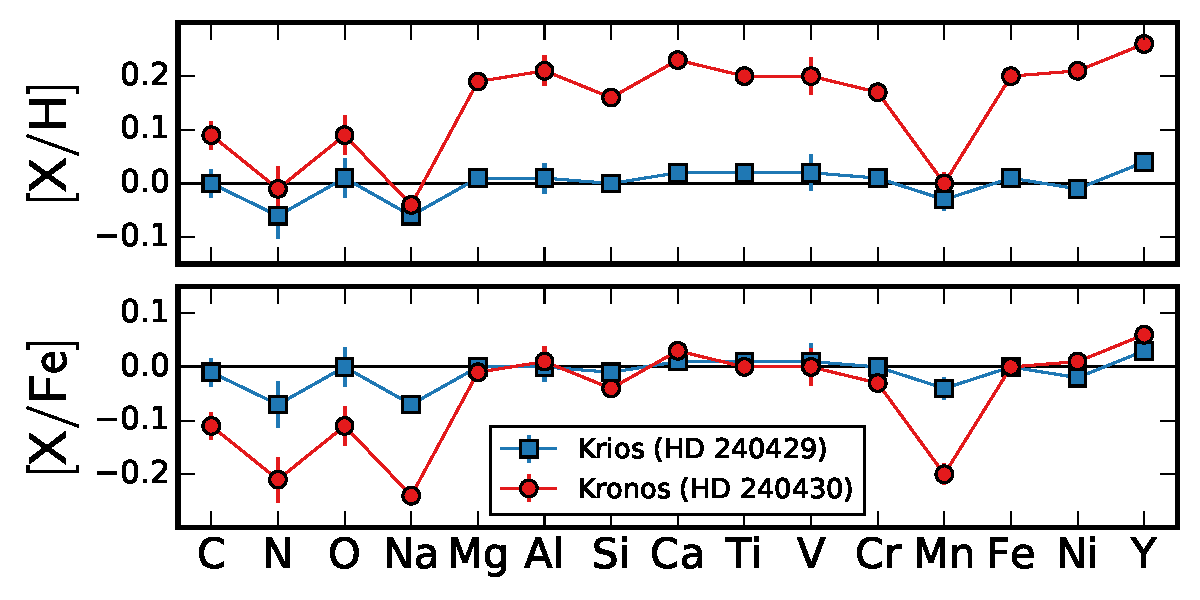
\includegraphics[width=0.9\linewidth]{abundances.pdf}
  \caption{Abundances of the co-moving pair, HD 240429 and HD 240430.}
  \label{fig:abundances}
\end{figure}

\begin{figure}[htpb]
  \centering
  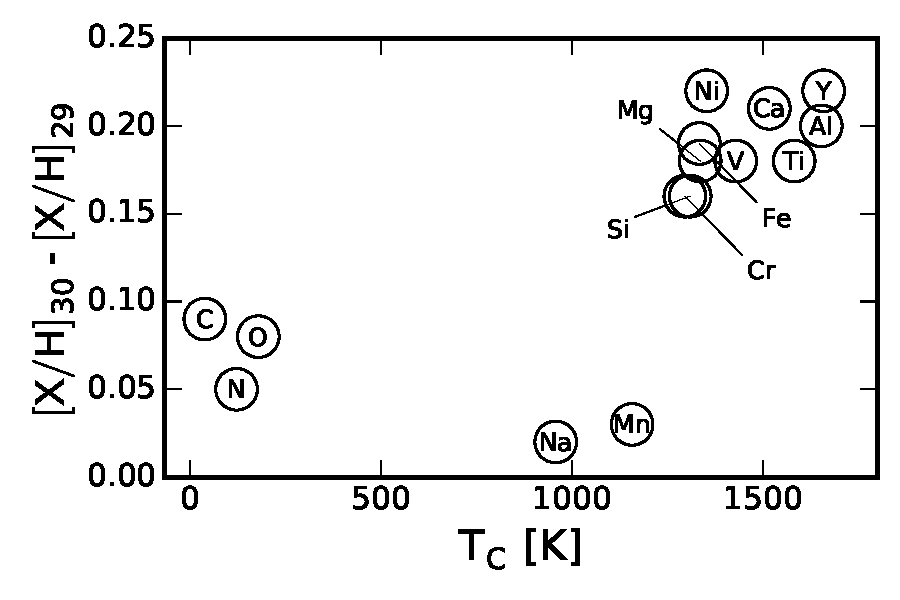
\includegraphics[width=0.9\linewidth]{relabun_tc_XH.pdf}
  \caption{Abundance of HD 240430 ($[\mathrm{Fe}/\mathrm{H}] = 0.20$)
    relative to HD 240429 ($[\mathrm{Fe}/\mathrm{H}] = 0.01$)
    as a function of condensation temperature of elements (\citealt{2003ApJ...591.1220L}).
  }
  \label{fig:relabun_tc}
\end{figure}

\section{Discussion}
\label{sec:discussion}

We discuss the possible origins of this pair.
Let us first consider scenarios in which the two stars are not actually born together.

% chance pair
Given that their metallicities and abundance patterns are significantly
different, one may simply conclude that the two stars are not related (coeval)
but they merely happen to be co-moving at such small separation ($\approx 0.6$~pc)
by chance.
The two stars are in the Galactic disk, and assuming certain velocity ellipsoid
at the stars' location, one may compute the probability that a star moving at
the mean velocity of the two stars would have a companion within $\Delta v = XX$~km/s.
...

% binary-single and binary-binary exchange
Another scenario that two unrelated stars may end up in a wide binary system
is multi-body gravitational scattering.
We consider the exchange probabilities in binary-single and binary-binary interactions.
Given their low binding energy compared to incoming velocity of field stars,
this is low.
Two factors that make this even more unlikely are that both stars are very young given their large Li,
and that if the pair is a result of scattering, one expect to end up with typical stars of the field,
not HD30 with anomalous abundance patterns.


None of the above scenarios is quite satisfactory as it offers no
insight on the peculiarity in abundances of HD 30 (see \ref{sec:data}).

The unlikeliness of the above possibilities naturally leads us to
consider the alternative.
What can selectively enrich XX elements in one of the two stars that are born together?

% inhomogeneity in star formation
It may be that the two stars are born at the same time from the same cloud, but
there is inhomogeneity. Highly doubtful based on
- Brewer et al. binaries that seem identical.
- other?

% rocky planets (or the like) engulfment
Yet another possibility is that the more metal-rich of the two stars
was recently? bombarded by something that selectively removed the depleted elements but not the others.

estimate: 10 earth mass

Present the relative abundance figure here

Change in stellar abundance due to ingestion of planets has been considered
for similar bright star pairs HD XX/XX (Mack) and HD XX/XX(Mack).


% Concluding remakrs


\bibliography{ref}



\end{document}
